\section{簡介}
在使用深層類神經網絡模型時,通常會讓訓練與測試時的環境設定標準一致,讓模型可以成功的學習並且應用在實務層面上。訓練時,模型從廣大、豐富甚至重複的資料中擷取關鍵資訊,結構化組織成模型的中間參數;測試時,模型通常有其核心目標,諸如分類器或是回歸器。根據不同的應用層面,測試時必須根據所學的知識,迅速或是正確的完成任務。

近年來,由於巨量數據與硬體資源的加速擴張,辛式(Hinton)提出知識蒸餾(Knowledge Distiilation, KD)的概念,把深層類神經網路的訓練期以及測試期的模型架構分開。在訓練期的時候,模型必須要有足夠強大的架構、參數,才能汲取足夠的資訊,形成厚重模型(Cumbersome Model)。針對厚重模型,設計者可以無所不用其極地使用高複雜度的優化演算法(Optimization Algorithm)、強力的控制調適子(Regularizer)、或是龐大的結合模型(Ensemble Model)來輔助訓練,讓模型可以充分學習到知識,同時保有概括化的能力。

然而厚重模型往往龐大,無法真正套用在即時(Real-time)的應用層面上。於是,利用額外一個小型、輕便、簡單的蒸餾模型(Distillation Model),將厚重模型所汲取的豐富知識,「蒸餾」給蒸餾模型。此命名取其細火慢燉、冷凝氣態精華之意,化用自化學實驗的定義:「藉由沸點的不同,選擇性地將液體混合物中的不同物質分離,萃取指定的物質。」

典型的知識蒸餾過程如下:

\begin{itemize}
\itemsep -2pt
 \item 根據豐富的訓練資料集,設定龐大的模型架構與複雜的優化演算法,訓練出厚重模型。
 \item 選定轉移資料集,可能就是訓練資料、經揀選過的精華資料或是根本沒有正確答案的非監督資料。
 \item 在轉移資料集上,將厚重模型學到的資訊,蒸餾給蒸餾模型。
\end{itemize} 

使用知識蒸餾訓練模型之前,必須先思考到底什麼樣的重要資訊,會潛藏在厚重模型裡面。考慮一個簡單的圖形數字分類器的例子,如圖\ref{fig:chap5_digit_classifier_example}。

\begin{figure}[!h]
\centering
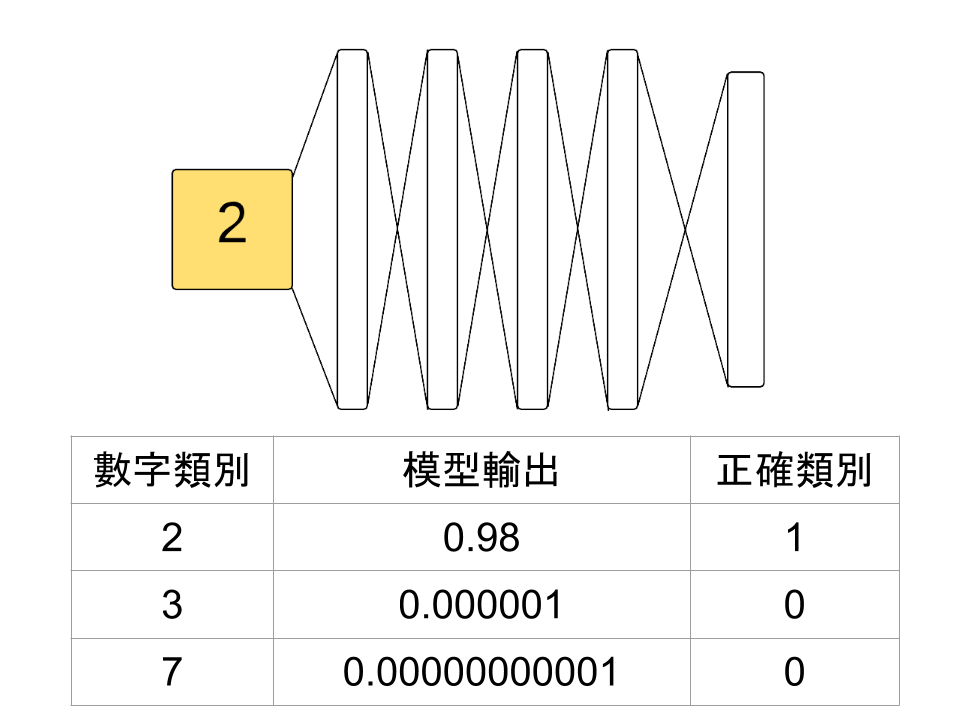
\includegraphics[scale=0.30]{images/chap5_digit_classifier_example.png}
\caption{一個簡單的深層類神經網路作為數字分類器。}
\label{fig:chap5_digit_classifier_example}
\end{figure}

假設這個分類器問題,在於分類數字2、3還有7。在訓練分類器時,給定的正確答案通常是1-hot向量,如$[1, 0, 0]$,明確地告知這張是數字為2的圖。

人類在學習的道路上,更追求舉一反三的概括化能力,因此我們可能會更想要機器知道,這張標示為2的圖,到底跟3比較像,還是跟7比較像。這樣的概括能力無法在1-hot的向量裡看到,因為向量裡兩個輸出的值皆為0,訓練目標裡,根本不期望模型能夠區分3和7與2這個數字的接近程度,因而與實際的學習目標:概括化能力有些差異。

根據此觀察,知識蒸餾的重點,便是希望厚重模型將其畢生所學的資訊,轉化為概括化的能力,傳授給蒸餾模型。如圖\ref{fig:chap5_digit_classifier_example}中,厚重模型的輸出向量為$[0.98 , 10^{-6} , 10^{-11}]$,不僅能夠學習到2的正確答案,亦能夠發現3比7還來得接近正解。

因應知識蒸餾的傳授特性,厚重模型學識淵博,亦可稱教師模型(Teacher Model),而蒸餾模型亦可稱學生模型(Student Model),取其師承同門之意。

\section{溫度軟性最大化(Temperature Softmax)}

化學蒸餾時,控制蒸餾過程能否有效萃取指定物質的關鍵,就是加熱溫度。溫度過高時,所有物質的汽化的比例越接近,沒有純化的功能;溫度過低,分子動能減低,蒸餾效率降低,甚至無法進行蒸餾萃取。

\begin{figure}[!h]
\centering
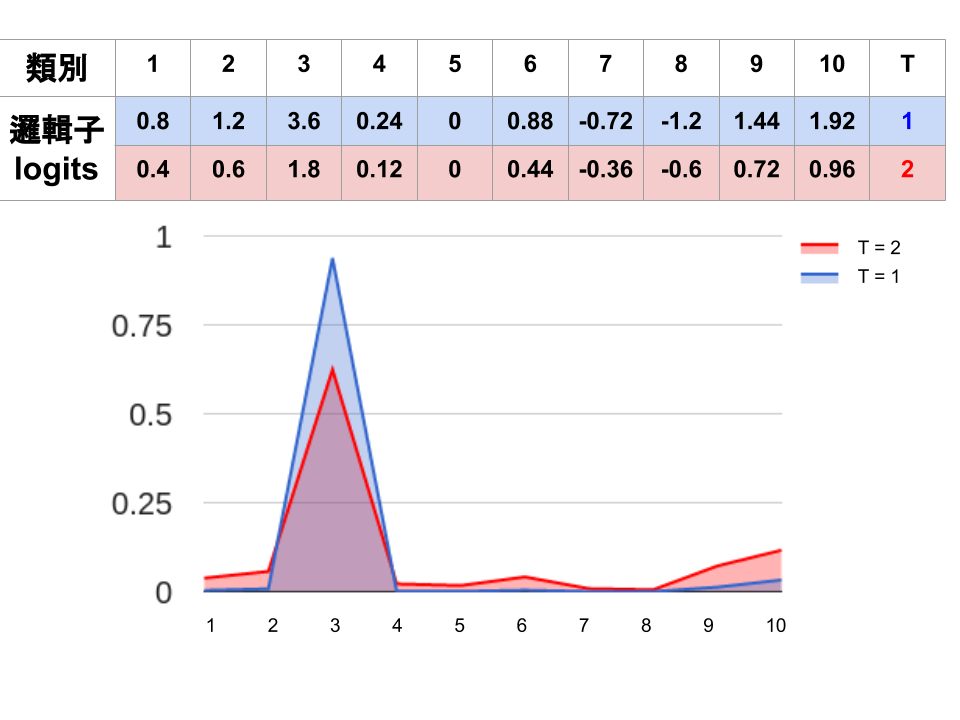
\includegraphics[scale=0.30]{images/chap5_impurity.png}
\caption{兩種經過溫度軟性最大化的機率分佈,藍線為無溫度,紅線為溫度2。}
\label{fig:chap5_impurity}
\end{figure}
在知識蒸餾時,亦有相同的議題存在。厚重模型必須把其輸出機率分布中隱含的概括化資訊,傳授給蒸餾模型。如圖\ref{fig:chap5_impurity}藍線,如果機率的分布越不平均,表示某些峰值的機率特別高,必然有重要的資訊存在,使得分類器能夠有所憑據地進行預測;然而,峰值以外的其他可能性差異變小,所包含的概括化資訊就越少。

一般分類器進行分類時,會使用如公式\ref{eq:softmax}的軟性最大化(Softamx)轉換,將邏輯子在對數空間中正規化成機率分布。

在知識蒸餾過程時,通常會使用更廣義的溫度軟性最大化(Temperature Softmax):
\begin{equation}
\hat{y}_i = \frac{e^{\frac{z_i}{T} }}{\sum_{k=1}^{C}e^{\frac{z_k}{T}} }
\end{equation}
其中,$T$是溫度。溫度並不會改變經過軟性最大化後各項機率的順序,但溫度越大,分布的不均度(Impurity)會下降,使得分布形狀稍微平坦一些,如圖\ref{fig:chap5_impurity}的紅線。

厚重模型如若經過高溫軟性最大化的轉換,便能提供更加軟性的輸出,凸顯潛藏在非正確類別之間的概括化資訊,以方便將資訊蒸餾給蒸餾模型。然而正確類別的機率卻會下降,是為權衡。

\section{蒸餾設定與步驟}

公式\ref{eq:LCE}裡,分類器的訓練損失函數為交叉熵,計算模型輸出與目標1-hot向量的克雷散度,是為硬式目標(Hard Target)。在知識蒸餾階段,則計算蒸餾模型輸出與厚重模型輸出的克雷散度,作為軟式目標(Soft Target),如公式\ref{eq:chap5_soft_target}。

\begin{equation} \label{eq:chap5_soft_target}
L_{KD}(x, \theta_{s} , \theta_{t} , T ) = KL( f_{\theta_{t} }^{T} || f_{\theta_{s}}^{T} )
\end{equation}
其中$\theta_{s}$是學生模型(蒸餾模型)的參數,$\theta_{t}$是教師模型(厚重模型)的參數,$T$是蒸餾過程中的軟性最大化轉換溫度。軟式目標旨在將厚重模型的概括化資訊,先經由溫度軟化後萃取給蒸餾模型。然而,厚重模型的輸出分佈可能不正確,為了補足萃取過程中遺失的正確類別資訊,較穩定的訓練方法是將硬式目標與軟式目標加權平均,作為整體的訓練目標:

\begin{equation}
L = \lambda \times L_{CE} + (1-\lambda) \times T^2 \times L_{KD}
\end{equation}
其中$\lambda$是硬式目標的比例,通常設定0.1。$T^2$項是為了補足溫度軟性最大化中,因為升溫而產生的數值縮小。

\section{多語言知識蒸餾}
知識蒸餾能夠將厚重的教師模型學到的概括化資訊,傳授給學生模型。這個概念與多語言語音辨識系統中,以深層類神經網路中間層合併的聲學模型中,互相借助語言學習到跨語言知識,有許多相似的部分。前者著重在垂直的模型強度,由教師模型傳授給學生模型;後者著重在平行的模型共享,不同語言之間合併訓練。

然而,多語言的訓練情景,由於藉助其他語言,往往陷入資料量爆炸的問題。不斷提升模型參數數量,提昇類神經網路中的寬度與深度,會讓模型有更多的潛能以學到跨語言知識,卻無法套用到實際應用上。因此,龐大的多語言厚重模型,需仰賴知識蒸餾,將所學的知識傳授給同樣是多語言情景訓練的學生模型。

多語言的知識蒸餾,有兩種可能的資訊包含在厚重模型中的概括化能力:
\begin{itemize}
 \itemsep -2pt
 \item 概括化資訊包含於厚重模型的輸出,是語言特定的分類資訊,因此使用單語言的教師模型進行蒸餾。
 \item 概括化資訊隱含聲音相似程度,是橫跨語言的特徵資訊,因此使用多語言的教師模型進行蒸餾。
\end{itemize}

其中,使用多個單語言教師模型同時進行蒸餾時,訓練方式如圖\ref{fig:chap5_multiple_monolingual_cumbersome}。使用單個多語言的教師模型進行蒸餾時,訓練方式如圖\ref{fig:chap5_single_multilingual_cumbersome}。
\begin{figure}[!ht]
\centering
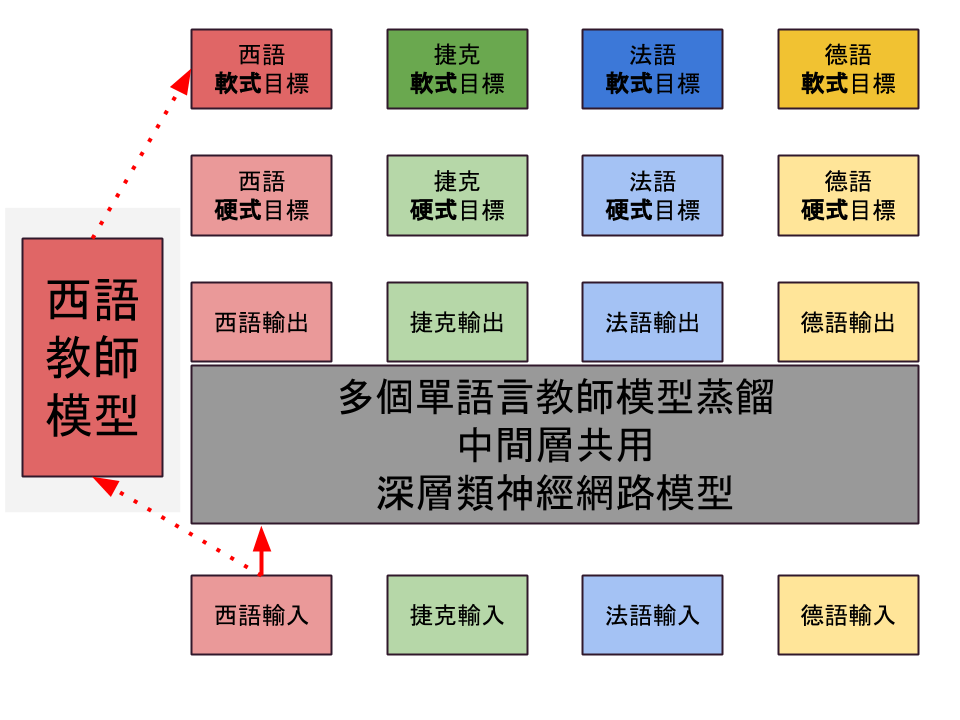
\includegraphics[scale=0.28]{images/chap5_multiple_monolingual_cumbersome.png}
\caption{以多個單語言教師模型進行知識蒸餾。圖中只有呈現西語的教師模型,然實際情形是四個教師模型共同發揮。}
\label{fig:chap5_multiple_monolingual_cumbersome}
\end{figure}

\begin{figure}[!ht]
\centering
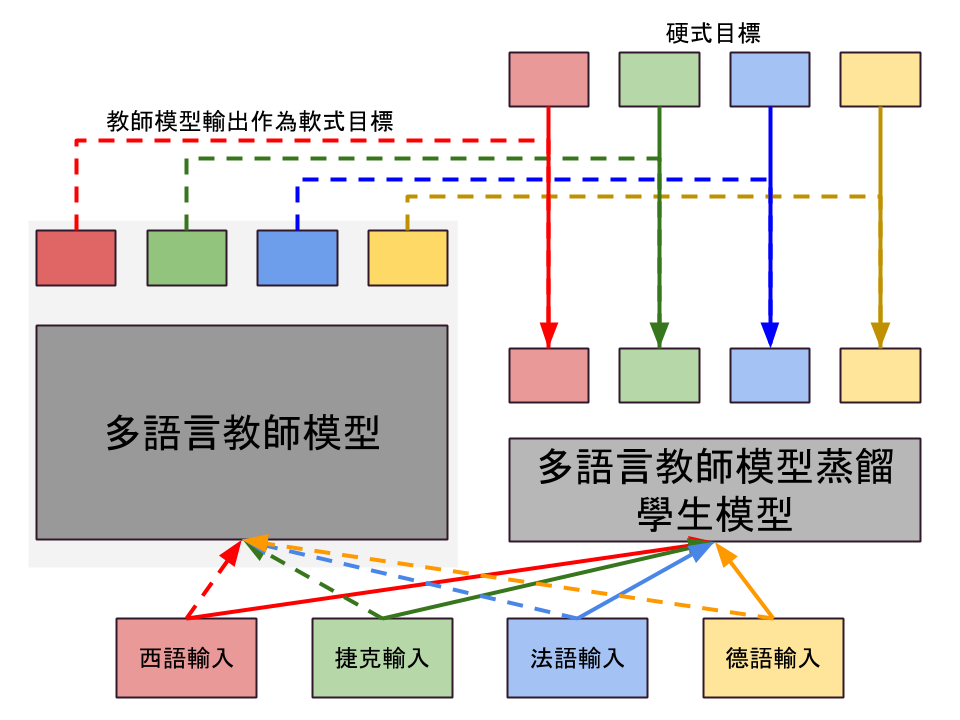
\includegraphics[scale=0.28]{images/chap5_single_multilingual_cumbersome.png}
\caption{以單個多語言教師模型進行知識蒸餾。}
\label{fig:chap5_single_multilingual_cumbersome}
\end{figure}

本章的研究目標是將知識蒸餾套用在多語言語音辨識系統中,借助垂直與水平的資訊整合,提升辨識成果。

%\section{蒸餾與模型壓縮}
\section{實驗結果與分析}
本章先實作四個語言的單語言知識蒸餾,再與多語言知識蒸餾結果比較。
\subsection{單語言知識蒸餾}
表\ref{table:chap5_monolingual_distillation},是GP語料庫中四個語言的單語言知識蒸餾實驗結果。表中有四組實驗數據,分別是單語言基準實驗(同表\ref{table:chap3_dropout})、7層線性整流子搭配丟棄演算法訓練成的單語言教師模型(同表\ref{table:chap3_depth})、4層線性整流子搭配丟棄演算法,經過教師模型知識蒸餾後的學生模型,以及同樣是4層線性整流子搭配演算法,但未經過蒸餾的模型。

\begin{table}[htbp]
%\resizebox{\columnwidth}{!}{
\centering
\begin{tabular}{|c>{\columncolor{red!20}}c>{\columncolor{green!20}}c>{\columncolor{blue!20}}c>{\columncolor{yellow!20}}c>{\columncolor{gray}}cc|}
\hline
 方法 & 西語 & 捷克 & 法語 & 德語 & AWERR & 參數數量 \\
\hline
  單語言基準實驗 & 8.74\% & 18.16\% & 17.43\% & 15.85\% & 100\% & 75.6M \\
  + 線性整流與丟棄0.1 & 8.58\% & 17.61\% & 17.15\% & 15.40\% & 97.67\% & 75.6M \\
\hline
  單語言教師模型 & 8.41\% & 17.03\% & 16.80\% & 14.50\% & 94.45\% & 126.4M \\
\hline
  單語言學生模型 & 8.20\% & 17.05\% & 16.80\% & 14.12\% & 93.26\% & 75.6M \\
\hline
\end{tabular}
\caption{單語言語音辨識中,使用知識蒸餾的詞誤率比較表格。表中的聲學模型都是使用寬度為2048神經元的深層類神經網路。}
\label{table:chap5_monolingual_distillation}
\end{table}

表\ref{tabele:chap5_monolingual_distillation}中,單語言學生模型的架構與單語言基準實驗加上線性整流與丟棄0.1的模型架構一模一樣,只差在是否接受教師模型的蒸餾。

然而,學生模型(AWERR 93.26\%)不僅擊敗以一般演算法進行學習的類神經網路(AWERR 97.67\%),甚至名師出高徒,在AWERR的表現上勝過教師模型(AWERR 94.45\%)。這表示:
\begin{itemize}
\itemsep -2pt
 \item 師傅亦是半途出家,7層的教師模型尚未發揮相等容量下極致的表現。
 \item 學生化用師傅所傳,青出於藍,4層的學生模型從硬式目標中獲得分類資訊又能夠從教師模型中獲得概括化能力,結合兩者因而表現的更好。
\end{itemize}

考量到參數數量,能夠發現單語言知識蒸餾成功地進行模型壓縮,讓學生模型有教師模型的辨識能力,參數數量又減少了40\%。這也證明了訓練深層類神經網路的區域極值問題,小模型擁有好表現的參數能力,只是訓練演算法未必能夠成功訓練到正確的位置上。

\subsection{多語言知識蒸餾}

表\ref{table:chap5_multilingual_distillation},是GP語料庫中四個語言的多語言知識蒸餾實驗結果,分別是單語言基準實驗(同表\ref{table:chap3_dropout})、單語言教師模型、7層中間層共享的多語言教師模型(同表\ref{table:chap4_dnn_sharing})、單語言教師蒸餾後的4層中間層共享多語言學生模型、多語言教師蒸餾後的4層中間層共享多語言學生模型、以及4層中間層共享但未經蒸餾的多語言模型。

\begin{table}[htbp]
%\resizebox{\columnwidth}{!}{
\centering
\begin{tabular}{|c>{\columncolor{red!20}}c>{\columncolor{green!20}}c>{\columncolor{blue!20}}c>{\columncolor{yellow!20}}c>{\columncolor{gray}}cc|}
\hline
 方法 & 西語 & 捷克 & 法語 & 德語 & AWERR & 參數數量 \\
\hline
  單語言基準實驗 & 8.74\% & 18.16\% & 17.43\% & 15.85\% & 100\% & 75.6M \\
  單語言教師模型 & 8.41\% & 17.03\% & 16.80\% & 14.50\% & 94.45\% & 126.4M \\
\hline
  多語言教師模型 & 8.10\% & 16.75\% & 16.65\% & 12.95\% & 90.38\% & 49.9M \\
  多語言4層共享中間層 & 8.29\% & 17.05\% & 16.93\% & 14.15\% & 93.74\% & 36.4M \\
\hline
  多個單語言教師蒸餾 & 8.14\% & 17.36\% & 16.86\% & 14.00\% & 93.39\% & 36.4M \\
  單個多語言教師蒸餾 & 7.90\% & 16.87\% & 16.96\% & 13.07\% & 90.60\% & 36.4M \\
\hline
\end{tabular}
\caption{多語言語音辨識中,使用知識蒸餾的詞誤率比較表格。表中的聲學模型都是使用寬度為2048神經元的深層類神經網路,只有基準實驗使用S型函數,其餘皆使用線性整流子丟棄0.1。}
\label{table:chap5_multilingual_distillation}
\end{table}

從表\ref{table:chap5_multilingual_distillation}中可以看到,相同參數下,無論是單個多語言教師蒸餾(AWERR 93.39\%)還是多個單語言教師蒸餾(AWERR 90.60\%),結果都比相同模型參數的多語言4層共享中間層(AWERR 93.74\%)來得較好。

然而,單語言教師模型(AWERR 94.45\%)表現本不如多語言4層共享中間層來得好,卻依然能夠進步,可見在多語言訓練情景下,依然有些資訊可以從單語言訓練的教師模型中蒸餾獲得。可是,這個進步量遠遠不如單個多語言教師模型進行蒸餾來得高。推究其原因,乃多語言教師模型本身足夠強(AWERR 90.38\%),早已從大量跨語言資料中汲取強大的知識,符合知識蒸餾的發展動機,成為龐大的厚重模型。

從實驗中發現,單語言教師蒸餾的方式,較能夠補足多語言共享中間層訓練中缺少的資訊,因此學生模型比起教師模型來得好,而多語言教師蒸餾則沒有此現象。但是更多的背景原因,在於多語言教師模型看到的資料量遠遠大於單語言教師模型,因而富含更多強力的資訊,使得學生模型無法超越。

知識蒸餾中,軟式目標的訓練方式非常近似於一般L2的二階控制調適子,藉由限制模型參數的成長範圍來避免過度貼合,卻又保有模型的分類潛力。端看公式,可能質疑如此的詞誤率進步來自於控制調適,而非教師模型中的額外資訊。

要觀察模型是否因為控制調適而獲得詞誤率的進步,可以觀察發展集上的音框準確度,如表\ref{table:chap5_dev_set_acc}。為了一致評比,亦使用了幾何平均來估算模型在四個語言發展集上的表現。可以發現,知識蒸餾有兩方面的意義顯現:
\begin{itemize}
 \itemsep -2pt
 \item 以單語言教師模型進行模型蒸餾後,發展集上的音框準確度(58.99\%)比同樣架構訓練而成的(60.84\%)來得低,但是測試集上的AWERR表現卻比較好。此種情形因為教師模型本身結果並不夠好,以輸出作為軟式目標的方法較接近控制調適。
 \item 以多語言教師模型進行模型蒸餾後,發展集上的音框準確度(62.40\%)比同樣架構訓練而成的(60.84\%)來得高,而且測試集上的AWERR也明顯表現得較好。此種情形下,教師模型本身能從跨語言資料中得到更多的資訊,而且能夠成功蒸餾給學生模型,不是控制調適。
\end{itemize}
\begin{table}[htbp]
%\resizebox{\columnwidth}{!}{
\centering
\begin{tabular}{|ccc|}
\hline
 方法 & 發展集上音框準確度幾何平均 & AWERR  \\
\hline
  單語言教師模型 & 58.22\% & 94.45\% \\
\hline
  多語言教師模型 & 62.82\% & 90.38\% \\
  多語言4層共享中間層 & 60.84\% &  93.74\% \\
\hline
  多個單語言教師蒸餾 & 58.99\% & 93.39\%  \\
  單個多語言教師蒸餾 & 62.40\% & 90.60\%  \\
\hline
\end{tabular}
\caption{多語言語音辨識中,使用知識蒸餾的實驗數據,用以比較知識蒸餾與控制調適。}
\label{table:chap5_dev_set_acc}
\end{table}

\subsection{蒸餾參數}
表\ref{table:chap5_nohard}中,呈現了兩組數據,一組純粹以軟式目標訓練,一組以1:9的比例(硬:軟)進行知識蒸餾。圖中可以驗證,教師模型進行蒸餾教學的時候,仍然需要憑借正確答案或真理來幫助訓練,否則教師模型本身的錯誤會讓學生模型無法學好。

\begin{table}[htbp]
%\resizebox{\columnwidth}{!}{
\centering
\begin{tabular}{|c>{\columncolor{red!20}}c>{\columncolor{green!20}}c>{\columncolor{blue!20}}c>{\columncolor{yellow!20}}c>{\columncolor{gray}}c|}
\hline
 方法 & 西語 & 捷克 & 法語 & 德語 & AWERR  \\
\hline
  多語言4層共享中間層 & 8.29\% & 17.05\% & 16.93\% & 14.15\% & 93.74\%  \\
\hline 
  加上硬式目標 & 8.13\% & 17.10\% & 16.97\% & 13.00\% & 91.45\%  \\
\hline
  純粹軟式目標 & 8.73\% & 17.78\% & 17.50\% & 14.88\% & 97.98\%  \\
\hline
\end{tabular}
\caption{多語言語音辨識系統中,使用知識蒸餾的詞誤率比較表格,表中除了第一組以外都是以單個多語言教師以溫度3進行蒸餾。所有數據使用的深層類神經網路模型都是4層2048,使用線性整流子以及丟棄0.1。}
\label{table:chap5_nohard}
\end{table}


表\ref{table:chap5_temperature}探討以單個多語言教師進行蒸餾時,設定不同時間參數$T$,各個學生模型的多語言語音辨識系統詞誤率比較。改變溫度對於實驗結果的差異頗大,如同化學蒸餾的程序一樣,溫度才是決定如何純化、萃取資訊的關鍵。表中的4組溫度設定,結果都比不使用知識蒸餾的4層共享中間層結果來得好。

\begin{table}[htbp]
%\resizebox{\columnwidth}{!}{
\centering
\begin{tabular}{|c>{\columncolor{red!20}}c>{\columncolor{green!20}}c>{\columncolor{blue!20}}c>{\columncolor{yellow!20}}c>{\columncolor{gray}}c|}
\hline
 溫度 & 西語 & 捷克 & 法語 & 德語 & AWERR  \\
\hline
  3 & 8.13\% & 17.10\% & 16.97\% & 13.00\% & 91.45\%  \\
\hline
  5 & 7.90\% & 16.87\% & 16.96\% & 13.07\% & 90.60\%  \\
\hline
  8 & 8.25\% & 17.11\% & 16.86\% & 13.81\% & 93.05\%  \\
\hline
  10 & 8.26\% & 17.08\% & 16.93\% & 13.99\% & 93.43\%  \\
\hline
\end{tabular}
\caption{多語言語音辨識中,使用不同溫度進行知識蒸餾的詞誤率比較表格。表中的設定情景皆與\ref{table:chap5_multilingual_distillation}的單個多語言教師蒸餾設定一致。}
\label{table:chap5_temperature}
\end{table}

%\subsection{模型壓縮}
\subsection{本章實驗總結}    

本章將知識蒸餾的萃取過程視為垂直式的資訊移轉,與多語言語音辨識系統下的水平式模型共享結合使用,試圖尋找更多的資訊幫助訓練。先以單語言的知識蒸餾,驗證知識蒸餾轉移概括化資訊的過程,如表\ref{table:chap5_monolingual_distillation},接著套用至多語言的知識蒸餾,如表\ref{table:chap5_multilingual_distillation}。兩者都能利用教師模型提供的概括化資訊,提昇辨識結果,使得相同4層的模型參數數量下,擁有接近甚至超過7層類神經網絡的預測能力。

然而多語言知識蒸餾有兩種可能,一種是借助多個單語言教師模型來蒸餾、另一種是借助單個多語言教師模型來蒸餾。前者本身的模型較難訓練地強大,因此蒸餾過程被視為另外一種型態的控制調適;後者成功的將大量知識的多語言教師模型,藉由知識蒸餾,傳授給參數數量少的學生模型。

本章亦討論了不同溫度下的知識蒸餾過程,以及是否加入硬式目標導正訓練,結果如表\ref{table:chap5_temperature}和表\ref{table:chap5_nohard}。調整不同溫度會改變萃取資訊的效果,但都會有所進步。而加入硬式目標顯然是必須的過程,不讓教師模型的錯誤破壞了學生模型的學習。


